%!TEX TS-program = xelatex
%\documentclass[]{resume}
\documentclass[]{resume}
\usepackage{graphicx}

\begin{document}

\graphicspath{ {images/} }

% --- Header --- %
\header{Michael }{Pobega}
       {Linux Systems Engineer}

% --- Footer --- %
\footer{References, Capstone documentation and personal projects available on request}

% --- Left Column --- %
\begin{aside}
%  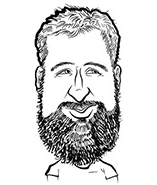
\includegraphics{caricaturesmall}
  \section{Contact}
    pobega@gmail.com
    (917) 436 - 0950
 \section{Skills}
    Linux system admin
    Programming
    Kernel debugging
    Application debugging
    Automation
  \section{Languages}
    Python
    Rust
    Perl
    Javascript
    Bash
    C/C++
  \section{Systems}
    ChromiumOS
    Gentoo
    Fedora/Silverblue
    Debian
    RedHat
    FreeBSD
  \section{Tools}
    Ansible, Nagios, Flatpak, Toolbox, Docker/Podman, nmap, Git, gdb, MongoDB, Virsh, Qemu, repo, Jenkins, Glade (GTK)
  \section{About Me}
    Passionate about desktop Linux, I'm interested in the future of containerized workflows via
    Toolbox and Flatpak.\break
    Other interests include
    fighting games, wine and horror movies.
  \section{Online}
    {\bodyfontbold pobega}.github.io
    github.com/{\bodyfontbold pobega}
    linkedin.com/in/{\bodyfontbold pobega}
    serverfault.com/{\bodyfontbold pobega}
\end{aside}

% --- Right Column --- %
\begin{main}
  \section{Work Experience}
    \experience{Neverware}{New York, NY}{Software Developer}{September 2016{\textasciitilde}Present}
      \point {Developer on Neverware's fork of ChromiumOS  "CloudReady"}
        \subpoint {Primarily focused on hardware compatibility and regression fixes}
      \point {Debugs and resolves hardware compatibility issues in CloudReady}
        \subpoint {Collaborates with Product and Sales to resolve customer issues}
        \subpoint {Manages driver compatibility and patches hardware quirks in the Linux kernel}
      \point {Merges upstream code back into Neverware's forks and resolves conflicts and build issues}
      \point {Maintains a Python tool to automate the creation of deployable CloudReady installer images}
        \subpoint {Saves Neverware's support team 2 hours per customer request}
      \point {Involved in company efforts to push relevant changes upstream}
        \subpoint {Upstreamed patches include Linux, Systemd, and HWDB}
    \experience{Neverware}{New York, NY}{Site Reliability Engineer}{September 2014{\textasciitilde}September 2016}
      \point {Administrator for Neverware's local Windows 7 Hypervisor solution "PCReady"}
        \subpoint {Managed roughly 300 PCReady servers across 120 schools}
      \point {Collaborated with the Engineering team to find and fix core product issues}
      \point {Engineered software in Python for monitoring and automation of PCReady tasks}
        \subpoint {\textit{TruancyOfficer} monitored server health and provided update emails}
        \subpoint {\textit{HallMonitor} alerted when servers were offline}
      \point {Handled customer support interactions for PCReady via phone and e-mail}
    \experience{SUNYIT CS/ITS Departments}{Utica, NY}{Linux System Administrator}{2010{\textasciitilde}2012, 2013{\textasciitilde}2014}
      \point {Responsible for the Gentoo Linux lab, as well as other misc. Linux labs on campus}
      \point {Implemented multicast ISO burning solution in Bash (\textit{wodimcast})}
      \point {Migrated services from legacy Unix hardware to a modern virtualized environment}
      \point {Reimplemented legacy mailing list software in Perl and integrate with existing LDAP}
      \point {Introduced configuration management through Ansible as a tool for rapid redeployment}
      \point {Setup Nagios server monitoring for the school's production network}
  \hrulefill
  \section{Education}
    \experience{SUNY Institute of Technology}{Utica, NY}{BSc Computer Science}{Class of May 2014}
      \point {Created an emulator for a fictional CPU architecture}
      \point {Wrote and booted a simplistic proof-of-concept x86 bootloader}
  \hrulefill
  \section{Personal Projects}
    \experience{Mullvad Indicator}{2020}{Gnome3 shell extension}{Gnome Javascript}
      \point {Monitor and control connectivity to the Mullvad.net VPN service}
    \experience{com.fightcade.Fightcade}{2020}{Fightcade application Flatpak}{YAML/Shell}
      \point {Sandboxes a proprietary application for easy distribution on Linux and CloudReady}
      \point {Bundles custom 32-bit Wine build for running Windows emulators on Linux}
\end{main}
\end{document}
